\documentclass{article}
\usepackage[margin=1in]{geometry}
\usepackage{amsmath,amsthm,amssymb}
\usepackage{bbm,enumerate,mathtools}
\usepackage{tikz,pgfplots}
\usepackage{chessboard}
\usepackage[hidelinks]{hyperref}
\usepackage{multicol} % Problem 35

\newenvironment{question}{\begin{trivlist}\item[\textbf{Question.}]}{\end{trivlist}}
\newenvironment{note}{\begin{trivlist}\item[\textbf{Note.}]}{\end{trivlist}}
\newenvironment{references}{\begin{trivlist}\item[\textbf{References.}]}{\end{trivlist}}
\newenvironment{related}{\begin{trivlist}\item[\textbf{Related.}]\end{trivlist}\begin{enumerate}}{\end{enumerate}}


\begin{document}
\rating{2}{2}
Let a palindromic partition be a partition of a string into palindromes.
\begin{figure}[!h]
  \centering
  % (x)(o)(x)(x)(o)
  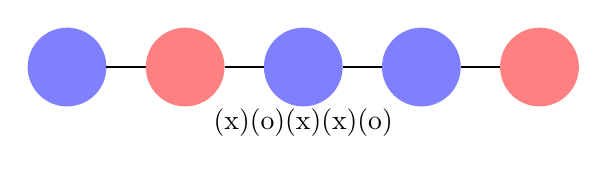
\begin{tikzpicture}
    \fill[blue!50] (0, 0) circle (0.5);
    \draw[thick] (0.5, 0)--(1, 0);
    \fill[red!50] (1.5, 0) circle (0.5);
    \draw[thick] (2, 0)--(2.5, 0);
    \fill[blue!50] (3, 0) circle (0.5);
    \draw[thick] (3.5, 0)--(4, 0);
    \fill[blue!50] (4.5, 0) circle (0.5);
    \draw[thick] (5, 0)--(5.5, 0);
    \fill[red!50] (6, 0) circle (0.5);
    \node at (3, -0.7) {(x)(o)(x)(x)(o)};
  \end{tikzpicture}\vspace{0.4cm}\\
  % (x)(o)(xx)(o)
  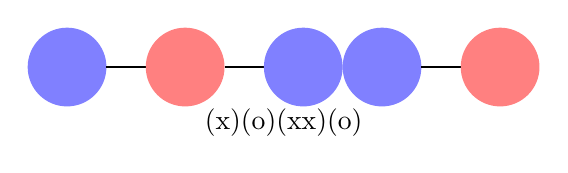
\begin{tikzpicture}
    \fill[blue!50] (0, 0) circle (0.5);
    \draw[thick] (0.5, 0)--(1, 0);
    \fill[red!50] (1.5, 0) circle (0.5);
    \draw[thick] (2, 0)--(2.5, 0);
    \fill[blue!50] (3, 0) circle (0.5);
    \fill[blue!50] (4, 0) circle (0.5);
    \draw[thick] (4.5, 0)--(5, 0);
    \fill[red!50] (5.5, 0) circle (0.5);
    \node at (2.75, -0.7) {(x)(o)(xx)(o)};
  \end{tikzpicture}\vspace{0.4cm}\\
  % (xox)(x)(o)
  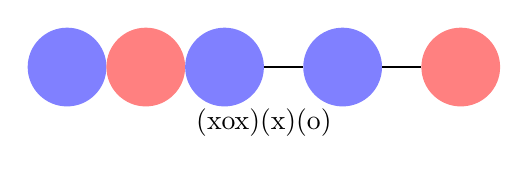
\begin{tikzpicture}
    \fill[blue!50] (0, 0) circle (0.5);
    \fill[red!50] (1, 0) circle (0.5);
    \fill[blue!50] (2, 0) circle (0.5);
    \draw[thick] (2.5, 0)--(3, 0);
    \fill[blue!50] (3.5, 0) circle (0.5);
    \draw[thick] (4, 0)--(4.5, 0);
    \fill[red!50] (5, 0) circle (0.5);
    \node at (2.5, -0.7) {(xox)(x)(o)};
  \end{tikzpicture}\vspace{0.4cm}\\
  % (x)(oxxo)
  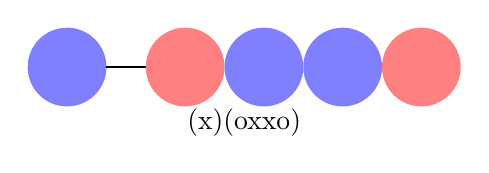
\begin{tikzpicture}
    \fill[blue!50] (0, 0) circle (0.5);
    \draw[thick] (0.5, 0)--(1, 0);
    \fill[red!50] (1.5, 0) circle (0.5);
    \fill[blue!50] (2.5, 0) circle (0.5);
    \fill[blue!50] (3.5, 0) circle (0.5);
    \fill[red!50] (4.5, 0) circle (0.5);
    \node at (2.25, -0.7) {(x)(oxxo)};
  \end{tikzpicture}
  \caption{
    An example of four palindromic partitions of the string ``xoxxo''.
  }
\end{figure}
\begin{question}
  Given some string, how many palindromic partitions does it have?
\end{question}
\begin{related}
  \item What is the least number of parts $p$ such that an arbitrary string of
    length $\ell$ over a $k$-letter alphabet can be partitioned into $p$ or
    fewer parts?
  \item What is the length of the shortest string that cannot be partitioned
    into fewer than $p$ parts?
  \item How many length $\ell$ strings require the ``worst-case'' number of
    parts?
  \item Which length $\ell$ strings have the greatest number of distinct
    partitions? The least?
  \item What is the smallest number of parts that any string with $m$ o's
    and an arbitrary number of x's can be partitioned into?
\end{related}
\begin{references}
  \item \url{https://oeis.org/A298481} the number of ways to partition the
    binary representation of n into the minimal number of palindromic parts.
\end{references}

\end{document}
